
% note-setup-borderless.tex
% fenglielie@qq.com 2025-07-10

\documentclass{article}
\usepackage{amsmath,amsthm,amsfonts,amssymb}
\usepackage{mathtools}
\usepackage{mathrsfs}
\usepackage{bm}
\usepackage{extarrows}
\usepackage[a4paper, margin=1in]{geometry}
\usepackage{float}
\usepackage{indentfirst}
\usepackage{anyfontsize}
\usepackage{booktabs,multirow,multicol}
\usepackage[shortlabels,inline]{enumitem}
\usepackage{appendix}

\usepackage[dvipsnames]{xcolor}
\usepackage{graphicx}
\graphicspath{
    {./figure/}{./figures/}{./image/}{./images/}{./graphic/}{./graphics/}{./picture/}{./pictures/}
}
\usepackage{subcaption}

\usepackage[ruled,linesnumbered,noline]{algorithm2e}
\usepackage{listings}
\lstdefinestyle{simpleStyle}{
    basicstyle=\ttfamily\small,
    breaklines=true,
    keywordstyle=\color{blue},
    identifierstyle=\color{black},
    stringstyle=\color{violet},
    commentstyle=\color[RGB]{34,139,34},
    showstringspaces=false,
    numbers=left,
    numbersep=2em,
    numberstyle=\footnotesize,
    frame=single,
    framesep=1em,
}
\lstset{style=simpleStyle}

\usepackage[colorlinks=true,linkcolor=,urlcolor=magenta,citecolor=violet]{hyperref}

\renewcommand*{\proofname}{\normalfont\bfseries Proof}

\usepackage{thmtools}
\usepackage{tikz}
\usepackage{tikz-3dplot}

%% define environments

\declaretheorem[style=plain, name=Theorem, numbered=yes, numberwithin=section]{theorem}
\declaretheorem[style=plain, name=Theorem, numbered=no]{theorem*}

\declaretheorem[style=plain, name=Proposition, numbered=yes, sibling=theorem]{proposition}
\declaretheorem[style=plain, name=Proposition, numbered=no]{proposition*}

\declaretheorem[style=plain, name=Corollary, numbered=yes, sibling=theorem]{corollary}
\declaretheorem[style=plain, name=Corollary, numbered=no]{corollary*}

\declaretheorem[style=plain, name=Lemma, numbered=yes, sibling=theorem]{lemma}
\declaretheorem[style=plain, name=Lemma, numbered=no]{lemma*}

\declaretheorem[style=plain, name=Claim, numbered=yes, sibling=theorem]{claim}
\declaretheorem[style=plain, name=Claim, numbered=no]{claim*}

\declaretheorem[style=definition, name=Definition, numbered=yes, numberwithin=section]{definition}
\declaretheorem[style=definition, name=Definition, numbered=no]{definition*}

\declaretheorem[style=definition, name=Example, numbered=yes, numberwithin=section]{example}
\declaretheorem[style=definition, name=Example, numbered=no]{example*}

\declaretheorem[style=definition, name=Problem, numbered=yes, numberwithin=section]{problem}
\declaretheorem[style=definition, name=Problem, numbered=no]{problem*}

\declaretheorem[style=remark, name=Remark, numbered=yes, numberwithin=section]{remark}
\declaretheorem[style=remark, name=Remark, numbered=no]{remark*}

\declaretheorem[style=remark, name=Note, numbered=yes, numberwithin=section]{note}
\declaretheorem[style=remark, name=Note, numbered=no]{note*}

\declaretheoremstyle[headfont=\bfseries, bodyfont=\normalfont, spaceabove=3pt, spacebelow=3pt, qed=\ensuremath{\square}]{solutionstyle}

\declaretheorem[style=solutionstyle, name=Solution, numbered=yes, numberwithin=section]{solution}
\declaretheorem[style=solutionstyle, name=Solution, numbered=no]{solution*}

\usepackage[most]{tcolorbox}

\newcommand{\newtcbenvironment}[2]{
    \tcolorboxenvironment{#1}{#2, enhanced, breakable, sharp corners, boxrule=0pt, colframe=white}
    \tcolorboxenvironment{#1*}{#2, enhanced, breakable, rounded corners, boxrule=0pt, colframe=white}
}

%% define styles

\newtcbenvironment{theorem}{colframe=RoyalPurple, colback=RoyalPurple!8}
\newtcbenvironment{proposition}{colframe=RoyalPurple, colback=RoyalPurple!8}
\newtcbenvironment{corollary}{colframe=NavyBlue, colback=SkyBlue!8}
\newtcbenvironment{lemma}{colframe=NavyBlue, colback=SkyBlue!8}
\newtcbenvironment{claim}{colframe=NavyBlue, colback=SkyBlue!8}

\newtcbenvironment{definition}{colframe=ForestGreen, colback=ForestGreen!5}
\newtcbenvironment{example}{colframe=RawSienna, colback=RawSienna!5}
\newtcbenvironment{problem}{colframe=WildStrawberry!30, colback=WildStrawberry!5}

\newtheorem{homework}{Homework}

%define short cut notation
\newcommand{\g}{\mathfrak{g}}
\newcommand{\h}{\mathfrak{h}}

\title{Riemann Surfaces}
\author{Zihan Ke}

\begin{document}
\maketitle

\section*{Introduction}
Riemann Surfaces is the one-dimensional complex manifold. Also, it can be described as the one-dimensional complex algeraic curves. I first encounter the concept of Riemann Surfaces in complex analysis.Later I found that Riemann Surfaces is not only an interesting object to learn itself. Since it cna be described as algebraic curves, it also provides a path to the study of algebraic geometry. I want to learn algebraic geometry and Riemann Surfaces is a good place to start. 
OUr goal in this note is to obtain Riemann-Roch theorem and its application.
\newpage

\section{Riemann Surfaces and complex \textbf{manifolds}.}
\subsection{holomorphic functions in 1-variable}
\subsection{holomorphic functions in $n$-variables}
\subsection{Complex \textbf{manifolds} \& Riemann Surfaces.}

\begin{definition}
    Let $X$ be a \textbf{topological} space.
    \begin{enumerate}
        \item A $n$-dim \textbf{complex} chart on $X$ is a \textbf{homeomorphism}
        \[
        \phi : U \xrightarrow{\cong} V \subset \mathbb{C}^n \text{ open}
        \]
        \item Two such charts are compatible if
        $U_1 \cap U_2 = \emptyset$ or $\phi_2 \circ \phi_1^{-1} \big| \phi_1 (U_1 \cap U_2)$ is holomorphic
        \item A $n$-dim complex atlas $\mathcal{A}$ is a collection of pairwise compatible charts on $X$.
        \item Two such atlases on $X$ are equivalent if $\mathcal{A} \cup \mathcal{B}$ is an atlas.
        \item A $n$-dim $\mathbb{C}$ \textbf{manifold} is a topological space (is Hausdorff \& $2^{\text{nd}}$ countable) with an equivalence class of $n$-dim $\mathbb{C} \text{ atlases}$.
        \item A Riemann surface is a $1$-dim $\mathbb{C}$ \textbf{manifold}.
    \end{enumerate}
\end{definition}

\textbf{Exercise :}
\begin{enumerate}
    \item Equivalence of atlases is an equivalence relation.
    \item $\exists$ unique maximal $\mathbb{C} \text{ atlas}$.
\end{enumerate}

\begin{remark}
    \begin{enumerate}[\upshape (i)]
        \item Refining an atlas doesn't change the complex structure.
        \item If $\phi : U \to V$ is a chart on Riemann Surface $X$.
        \[
        \alpha : V \xrightarrow{\wedge} W
        \]
        then $\alpha \circ \phi : U \to W$ is a chart compatible with $\phi$.
        \item An $n$-dimensional \textbf{manifold} is a $2n$-dimensional real smooth \textbf{manifold}.
    \end{enumerate}
\end{remark}

\subsection{Examples of Riemann Surfaces.}

\begin{example}
\begin{enumerate}
    The first example is a \textbf{Non-Examples:} 
    \item $X = \mathbb{R}^2 \times U \to V = \mathbb{C}$ for $i=1, 2$.
    \begin{align*}
        \phi_1 (x, y) &= x + iy \\
        \phi_2 (x, y) &= \frac{x+iy}{1+i dx^2 y^2}
    \end{align*}
    $\phi_1$ \& $\phi_2$ are not compatible.
    $\phi_2 \circ \phi_1^{-1} (z) = \frac{z}{1+|z|^2}$ not holomorphic.
    \item The complex plane $\mathbb{C}$.
    $X = \mathbb{R}^2$. with $\phi_1 : \mathbb{R}^2 \to \mathbb{C}$.
    \[
    (x, y) \mapsto x+iy
    \]
    is a Riemann Surface.
    \item The Riemann Sphere. $\mathbb{CP}^1$:
    $X = S^2 = \{ (x, y, z) \in \mathbb{R}^3 : x^2 + y^2 + z^2 = 1 \} \subset \mathbb{R}^3$.
    (the stereographic projection with some modifications)
\end{enumerate}
\end{example}

%there should be a image of steoregraphic projection
\begin{figure}[h!] % The [h!] is an optional placement specifier
    \centering % This centers the drawing on the page
    \tdplotsetmaincoords{70}{110}
    \begin{tikzpicture}[tdplot_main_coords, scale=2]

        % Sphere
        \draw[ball color=cyan, opacity=0.4] (0,0,0) circle (1);

        % Projection plane
        \fill[gray, opacity=0.2] (-2,-2,-1) -- (2,-2,-1) -- (2,2,-1) -- (-2,2,-1) -- cycle;
        \draw (-2,-2,-1) -- (2,-2,-1) -- (2,2,-1) -- (-2,2,-1) -- cycle;
        \node at (2, -2, -1) [below right] {$z=-1$};

        % North pole (projection point)
        \fill[red] (0,0,1) circle (0.05);
        \node at (0,0,1) [above] {$N$};

        % Point on the sphere
        \tdplotsetthetaplanecoords{60}{30}
        \tdplotdrawarc[tdplot_rotated_coords, thick, red]{(0,0,0)}{1}{0}{360}{}{}
        \tdplotsetthetaplanecoords{60}{30}
        \coordinate (P) at (1,0,0);
        \node at (P) [above right, red] {$P$};
        \fill[red] (P) circle (0.05);

        % Projection line
        \draw[dashed, blue] (0,0,1) -- (P);

        % Projected point on the plane
        \pgfmathsetmacro{\px}{1*cos(30)*sin(60)}
        \pgfmathsetmacro{\py}{1*sin(30)*sin(60)}
        \pgfmathsetmacro{\pz}{1*cos(60)}
        \pgfmathsetmacro{\pxprime}{2*\px/(1-\pz)}
        \pgfmathsetmacro{\pyprime}{2*\py/(1-\pz)}

        \coordinate (Pprime) at (\pxprime, \pyprime, -1);
        \fill[blue] (Pprime) circle (0.05);
        \node at (Pprime) [below, blue] {$P'$};
        \draw[dashed, blue] (P) -- (Pprime);
        \draw[blue, ->] (0,0,1) -- (Pprime);

        % Axes
        \draw[-latex] (0,0,0) -- (2,0,0) node[anchor=north east]{$x$};
        \draw[-latex] (0,0,0) -- (0,2,0) node[anchor=north west]{$y$};
        \draw[-latex] (0,0,0) -- (0,0,2) node[anchor=south]{$z$};

    \end{tikzpicture}
    \caption{An illustration of the stereographic projection.}
    \label{fig:stereo_proj}
\end{figure}
$S^2 \setminus \{ (0,0,1) \}$
\begin{align*}
    \phi_0 : U_0 &\longrightarrow V_0 = \mathbb{C} \\
    \parallel \\
    S^2 \setminus \{ (0, 0, 1) \} \\
    (x, y, w) &\longmapsto \frac{x+iy}{1-w} \quad \Rightarrow \quad \text{this is the stereographic projection}
\end{align*}
\begin{align*}
    \phi_{\infty} : U_{\infty} &\xrightarrow{\cong} V_{\infty} = \mathbb{C} \\
    \parallel \\
    S^2 \setminus \{ (0, 0, -1) \} \\
    (x, y, w) &\longmapsto \frac{x-iy}{1+w}
\end{align*}

\textbf{Exercise :} check these are charts.

$\phi_0$ \& $\phi_{\infty}$ are compatible. On $U_0 \cap U_{\infty} = S^2 \setminus \{ (0,0,1), (0,0,-1) \}$, $\phi_0(U_0 \cap U_{\infty}) \subset \mathbb{C}^* \subset V_0$.

$$
\frac{1}{\phi_0(x, y, w)} = \frac{1-w}{x+iy} = \frac{(1-w)(x-iy)}{x^2+y^2} = \frac{(1-w)(x-iy)}{1-w^2} = \frac{x-iy}{1+w} = \phi_{\infty}(x, y, w)
$$

Thus,
$$
\phi_{\infty} \circ \phi_0^{-1} (z) = \frac{1}{z} \text{ on } \mathbb{C}^* = \phi_0 (U_0 \cap U_{\infty}) \subset \mathbb{C} = V_0.
$$
holomorphic

Hence, $\{ \phi_0, \phi_{\infty} \}$ are an atlas, and the corresponding Riemann Surface is called the **Riemann Sphere**.

\begin{enumerate}
    \item **Complex tori of dimension 1.**
    For $\omega_1, \omega_2 \in \mathbb{C}$ which are $\mathbb{R}$-linearly independent. consider the lattice $L = \mathbb{Z}\omega_1 + \mathbb{Z}\omega_2 = \{ n\omega_1 + m\omega_2 : n, m \in \mathbb{Z} \} \subset \mathbb{C}$.
    Let $X = \mathbb{C}/L$, with the quotient topology.
$$
\pi : \mathbb{C} \longrightarrow X = \mathbb{C}/L.
$$
$$
z \longmapsto [z] = z+L.
$$
Topologically $X$ is a torus.

Every $z \in \mathbb{C}$ is equivalent to a unique point in the
Fundamental domain.

\begin{center}
    % Placeholder for the fundamental domain parallelogram
    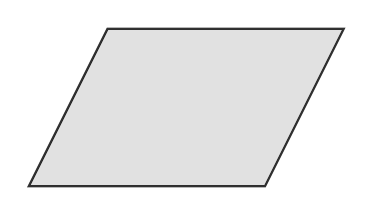
\begin{tikzpicture}
        \coordinate (A) at (0, 0);
        \coordinate (B) at (3, 0);
        \coordinate (C) at (4, 2);
        \coordinate (D) at (1, 2);
        \draw[thick, fill=gray!30, opacity=0.8] (A) -- (B) -- (C) -- (D) -- cycle;
    \end{tikzpicture}
\end{center}

Given $X = \mathbb{C}/L$, we construct an atlas using $\pi : \mathbb{C} \to \mathbb{C}/L$.

Pick $\varepsilon > 0$ s.t. $\forall p \in \mathbb{C}$, $B_{\varepsilon}(p)$ intersects each $[z]$ in at most one point.

Thus gives a homeomorphism
$$
\pi : B_{\varepsilon}(p) \xrightarrow{\cong} \pi(B_{\varepsilon}(p))
$$
$$
\text{with } \phi_p = \pi \big|_{B_{\varepsilon}(p)} : U_p \subset X
$$
where $U_p = \pi(B_{\varepsilon}(p))$.

\textbf{Claim :}
$$
\mathcal{A} = \{ \phi_p : U_p \to V_p \}_{p \in \mathbb{C}} \text{ is an atlas.}
$$

Compatibility of $\phi_p$ \& $\phi_q$:
Assume $U_{p, q} = U_p \cap U_q \neq \emptyset$.

The transition map is:
$$
T = \phi_q \circ \phi_p^{-1} : \phi_p(U_{p, q}) \longrightarrow \phi_q(U_{p, q})
$$
$T$ satisfies $\pi(T([z])) = \phi_p^{-1}([z]) = \pi([z])$ i.e., $T([z])-z \in L = \ker(\pi)$, which is constant.
$$
\Rightarrow T - \mathrm{id} \text{ is locally constant: locally } T - \mathrm{id} = w \in L.
$$
$$
T(z) = z + w \text{ is holomorphic}
$$
\end{enumerate}

\begin{center}
    % Placeholder for the diagram showing C mapping to X=torus
    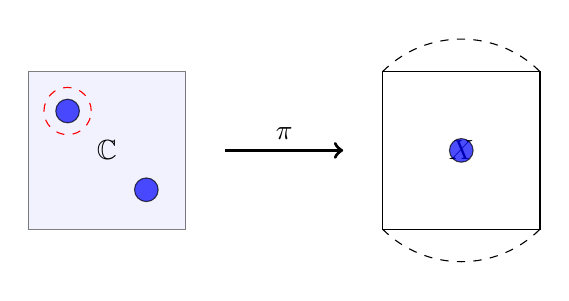
\begin{tikzpicture}
        % C plane (source)
        \draw[fill=blue!10, opacity=0.5] (-3, -0.5) rectangle (-1, 1.5);
        \node at (-2, 0.5) {$\mathbb{C}$};

        % X torus (target)
        \draw (1.5, -0.5) -- (3.5, -0.5) -- (3.5, 1.5) -- (1.5, 1.5) -- cycle;
        \draw[dashed] (1.5, 1.5) to[out=45, in=135] (3.5, 1.5);
        \draw[dashed] (1.5, -0.5) to[out=-45, in=-135] (3.5, -0.5);
        \node at (2.5, 0.5) {$X$};

        % Map pi
        \draw[->, very thick] (-0.5, 0.5) -- (1, 0.5) node[midway, above] {$\pi$};

        % Circles/points (covering map visualization)
        \draw[fill=blue, opacity=0.7] (-2.5, 1.0) circle (0.15);
        \draw[fill=blue, opacity=0.7] (-1.5, 0.0) circle (0.15);
        \draw[fill=blue, opacity=0.7] (2.5, 0.5) circle (0.15);
        \draw[dashed, red] (-2.5, 1.0) circle (0.3);
    \end{tikzpicture}
\end{center}

\subsection{Examples of complex \textbf{manifolds}.}

\begin{example}[Complex Projective Plane]
$$
\mathbb{CP}^n = \{ \text{1-dimensional complex vector subspace in } \mathbb{C}^{n+1} \} = \mathbb{C}^{n+1} \setminus \{ 0 \} / \mathbb{C}^*.
$$
$$
\cong S^{2n+1} / S^1 \quad \text{ quotient topology.}
$$

Give $\mathbb{CP}^n$ the quotient topology.
$$
\pi : \mathbb{C}^{n+1} \setminus \{ 0 \} \longrightarrow \mathbb{CP}^n
$$
$$
(z_0, \dots, z_n) \longmapsto \pi(z_0, \dots, z_n) = [z_0 : z_1 : \dots : z_n].
$$
homogeneous coordinates.

\textbf{Atlases:}
Let
$$
U_i = \{ [z_0 : \dots : z_n] : z_i \neq 0 \} \subset \mathbb{CP}^n \quad \text{ open}
$$
The chart $\phi_i$ is given by:
$$
\phi_i : U_i \longrightarrow V_i = \mathbb{C}^n
$$
$$
[z_0 : \dots : z_n] \longmapsto \left( \frac{z_0}{z_i}, \frac{z_1}{z_i}, \dots, \widehat{\frac{z_i}{z_i}}, \dots, \frac{z_n}{z_i} \right)
$$
where $\widehat{\frac{z_i}{z_i}}$ denotes the omission of the $i$-th coordinate.
\end{example}

\section{Morphisms of complex \textbf{manifolds} \& meromorphic functions.}

\subsection{Morphisms of \textbf{manifolds}.}

\begin{definition}
    Let $X$ \& $Y$ be complex \textbf{manifolds} of dimensions $n$ \& $m$ respectively.
    Let $W \subset X$ \& $W' \subset Y$ be open sets.
    \begin{enumerate}
        \item A continuous map $F: W \to W'$ is holomorphic at $p \in W$
        if $\exists$ charts $\phi : U \to V$ \& $\psi : W' \to V'$ s.t. $p \in U$
        \& $F(p) \in W'$, s.t. $\psi \circ F \circ \phi^{-1}$ is holo at $\phi(p)$.
        \item Biholomorphism.
    \end{enumerate}
\end{definition}

\begin{example}(Examples of Morphisms)
\begin{enumerate}
    \item A chart on a Riemann Surface $\phi : U \to V \subset \mathbb{C}$ on a Riemann Surface is a holomorphic function.
    \item Let $U \subset X$ for a Riemann Surface $X$. Then $U$ has a unique Riemann Surface structure s.t. the inclusion map $U \hookrightarrow X$ is holomorphic.
    \item Let $\mathbb{C}_{\infty} = \mathbb{C} \cup \{\infty\} \cong S^2 = U_0 \cup U_{\infty}$.
    Let $f$ be a holomorphic function on $\mathbb{C}$.
    Let $f_0 := f \circ \phi_0^{-1} : \mathbb{C} \to \mathbb{C}$.
    Let $f_{\infty} := f \circ \phi_{\infty}^{-1} : \mathbb{C} \to \mathbb{C}$.
On $\mathbb{C}^*$:
$$
f_{\infty}(w) = f \circ \phi_{\infty}^{-1}(w) = f \circ \phi_0^{-1} \circ \phi_0 \circ \phi_{\infty}^{-1}(w) = f_0 \left(\frac{1}{w}\right)
$$

This $f$ is holomorphic at $w \in \mathbb{C}_{\infty}$
$$
\iff f\left(\frac{1}{z}\right) \text{ is holomorphic at } 0
$$
$$
\Updownarrow \text{ Def}
$$
$$
f_{\infty}(w) \text{ is holomorphic at } 0 \iff f_0 \left(\frac{1}{w}\right) \text{ is holomorphic at } \infty
$$
 \item the quotient map $\pi: \mathbb{C}^n \to \mathbb{C}^n/L$ for a complex torus is holomorphic.
\end{enumerate}
\end{example}

subsection*{$\S$ 2.2. Properties of holomorphic maps of Riemann Surfaces.}

\begin{theorem}[The identity theorem] \label{thm:identity}
    Let $F, G: X \to Y$ be holomorphic maps of Riemann Surfaces s.t. $F$ \& $G$ agree on a subset of $X$ with an accumulation point.
    Then $F=G$.
\end{theorem}

\begin{theorem}[Local form of holomorphic maps] \label{thm:localform}
    Let $F: X \to Y$ be a non-constant holomorphic map of Riemann Surfaces.
    For $p \in X$ \& $q = F(p)$, $\exists$ unique $k \in \mathbb{Z}_{>0}$ and local charts $\phi : U \to V$ \& $\psi : U' \to V'$
    s.t. $F$ has local form
    $$
    \psi \circ F \circ \phi^{-1} : V \to V'
    $$
    $$
    z \mapsto z^k.
    $$
\end{theorem}

\begin{proof} 
    take any charts $\phi: U \to V \subset \mathbb{C}$ \& $\psi: U' \to V' \subset \mathbb{C}$.
$$
\begin{array}{ccc}
    X & \xrightarrow{F} & Y \\
    \downarrow{\phi} & & \downarrow{\psi} \\
    \mathbb{C} & \xrightarrow{f} & \mathbb{C}
\end{array}
\quad
\begin{array}{l}
    p \mapsto 0. \\
    q \mapsto 0.
\end{array}
$$

Shrink $V$ so $F(U) \subset U'$. Then $f = \psi \circ F \circ \phi^{-1} : V \to V'$
is holomorphic and $0 \mapsto 0$.

Define $k = \mathrm{ord}_0(f) \in \mathbb{Z}_{\ge 0}$. $\mathrm{ord}_0(f)$ is the order of vanishing of $f$
at $0 = \min \{ n \mid c_n \neq 0 \}$ where $f(z) = \sum_{n \ge 0} c_n z^n$ is
the Taylor expansion. $f(z) = z^k g(z)$, where $g(z)$ is non-zero.

Shrink $V$ so $g: V \to \mathbb{C}$ is non-zero and holomorphic.
Thus, $\exists$ holomorphic $k^{\text{th}}$ root $h: V \to \mathbb{C}$ of $g$
i.e., $(h(z))^k = g(z)$.

Thus $f(z) = z^k g(z) = (z h(z))^k$.

Let $\alpha : V \xrightarrow{\cong} \alpha(V)$ be biholomorphic
$$
z \mapsto z h(z) = w.
$$
Note $\alpha(0) = 0$, $\alpha'(0) = h(0) \neq 0$, then $\mathrm{ord}_0(\alpha) = 1$.

Now replace $\phi$ by $\alpha \circ \phi$.
$$
\psi \circ F \circ (\alpha \circ \phi)^{-1}(w) = \psi \circ F \circ \phi^{-1} \circ \alpha^{-1}(w)
$$
$$
= f(\alpha^{-1}(w)) = (\alpha^{-1}(w) h(\alpha^{-1}(w)))^k = w^k.
$$
Local form is $w \mapsto w^k$.
\end{proof}

\textbf{Exercise:}
Show $k$ is independent of the choice of chart.

\begin{definition}
    The \textbf{multiplicity} of a non-constant holomorphic map $F: X \to Y$
    of Riemann Surfaces at $p \in X$ is the unique positive integer $k$ given by
    Theorem 2.2.
\end{definition}

We say $p$ is an \underline{unramified point} of $F$ if $\mathrm{mult}_p(F) = 1$.
$p$ is a \underline{ramified point} of $F$ if $\mathrm{mult}_p(F) > 1$.

$$
R(F) = \{ p \in X : \mathrm{mult}_p(F) > 1 \} \text{ ramification locus.}
$$
$$
B(F) = F(R(F)) \subset Y \text{ branch locus.}
$$

\begin{theorem}[Open mapping theorem] \label{thm:openmapping}
    A non-constant holomorphic map of Riemann Surfaces is an open mapping.
\end{theorem}

\textbf{Proof:} The local form $z \mapsto z^k$ is open
("maps circle to circle").

\begin{theorem}[Biholomorphic maps are biholomorphisms] \label{thm:biholo}
    The inverse of a bijective holomorphic map of Riemann Surfaces is holomorphic
    (since $F$ is an open mapping).
\end{theorem}
\end{document}